% Nagłówek spisu załączników
\chapter*{Spis załączników}
\addcontentsline{toc}{chapter}{Spis załączników}

% Przełączenie w tryb załączników
\appendix
\renewcommand{\chaptername}{Załącznik}

% Ręczny spis załączników z hiperłączami do odpowiednich rozdziałów
\begin{description}
  \item[Załącznik A] \nameref{app:instrukcja}
  \item[Załącznik B] \nameref{app:formularz}
  \item[Załącznik C] \nameref{app:materialy}
\end{description}

% Pierwszy załącznik
\chapter{Tekstowa instrukcja przygotowania systemu pod kolejną edycję}
\label{app:instrukcja}
\headingformat{Wymagane programy i dostępy}
\begin{itemize}
    \item Przeglądarka internetowa
    \item Microsoft Excel (zalecana wersja desktopowa)
    \item Dostęp do kanału Inkubator\_PW na OneDrive
\end{itemize}

\headingformat{Przygotowanie bazy danych w Excel}
\textbf{Strona internetowa:} OneDrive Politechniki
\begin{enumerate}
    \item Zaloguj się na OneDrive przy użyciu danych konta Politechniki Warszawskiej.
    \item Przejdź do kanału "Inkubator\_PW" \href{https://wutwaw.sharepoint.com/sites/Inkubator_PW/Shared%20Documents/Forms/AllItems.aspx}{Kanał Inkubator\_PW}.
    \item Otwórz folder "Scientrepreneur's Club".
    \item Otwórz podfolder "Rejestracja z kanału Inkubatora".
    \item Znajdź plik \textbf{SC BAZA.xlsx} i otwórz go w Microsoft Excel.
    \item Skopiuj tabelę drugiej edycji i wklej ją w nowej zakładce.
    \item Zmień nazwę zakładki na "Tabela nr (numer edycji)".
    \item Usuń zawartość tabeli, zachowując nagłówki.
    \item Sprawdź formatowanie:
    \begin{itemize}
        \item Struktura kolumn musi być identyczna jak w poprzedniej edycji.
        \item Daty powinny być w formacie \textbf{dzień/miesiąc/rok}.
    \end{itemize}
    \item Zapisz plik i zamknij Excel.
\end{enumerate}

\headingformat{Przygotowanie formularza rejestracyjnego}
\textbf{Strona internetowa:} Microsoft Forms
\begin{enumerate}
    \item Otwórz przeglądarkę i przejdź na stronę \href{https://forms.office.com}{Microsoft Forms}.
    \item Zaloguj się danymi konta Politechniki Warszawskiej.
    \item Znajdź formularz z poprzedniej edycji i wybierz "Duplikuj".
    \item Zmień nazwę formularza na aktualną edycję.
    \item Edytuj treść (prelegent, temat, data).
    \item Skopiuj link do formularza i zapisz go.
\end{enumerate}

\headingformat{Konfiguracja automatycznego zapisu odpowiedzi}
\textbf{Strona internetowa:} Power Automate
\begin{enumerate}
    \item Zaloguj się na \href{https://flow.microsoft.com}{Power Automate}.
    \item Wybierz "Moje przepływy" > "Nowy przepływ" > "Automatyczny - od podstaw".
    \item Wpisz nazwę: "SC Edycja (numer edycji) - Automatyzacja".
    \item Wybierz wyzwalacz "Gdy nowa odpowiedź zostanie przesłana" (Microsoft Forms).
    \item Dodaj akcję "Pobierz szczegóły odpowiedzi".
    \item Dodaj akcję "Dodaj wiersz do tabeli" w Excel, wybierz plik \textbf{SC BAZA.xlsx}.
    \item Mapuj kolumny odpowiednio.
    \item Zapisz i przetestuj przepływ.
\end{enumerate}

\headingformat{Automatyzacja danych w Power Query}
\textbf{Program:} Power Query (Excel)
\begin{enumerate}
    \item Otwórz plik \textbf{SC BAZA.xlsx}.
    \item Wybierz \textbf{Dane} > \textbf{Edytor zapytań}.
    \item Znajdź istniejące połączenia (Tabela 1, kolejne tabele).
    \item Dodaj nowe zapytanie do odpowiedniego pliku na OneDrive.
    \item Połącz nowe zapytanie z główną bazą.
    \item Kliknij \textbf{Zamknij i załaduj}.
\end{enumerate}

% Drugi załącznik
\chapter{Formularz rejestracyjny na drugą edycję}
\label{app:formularz}
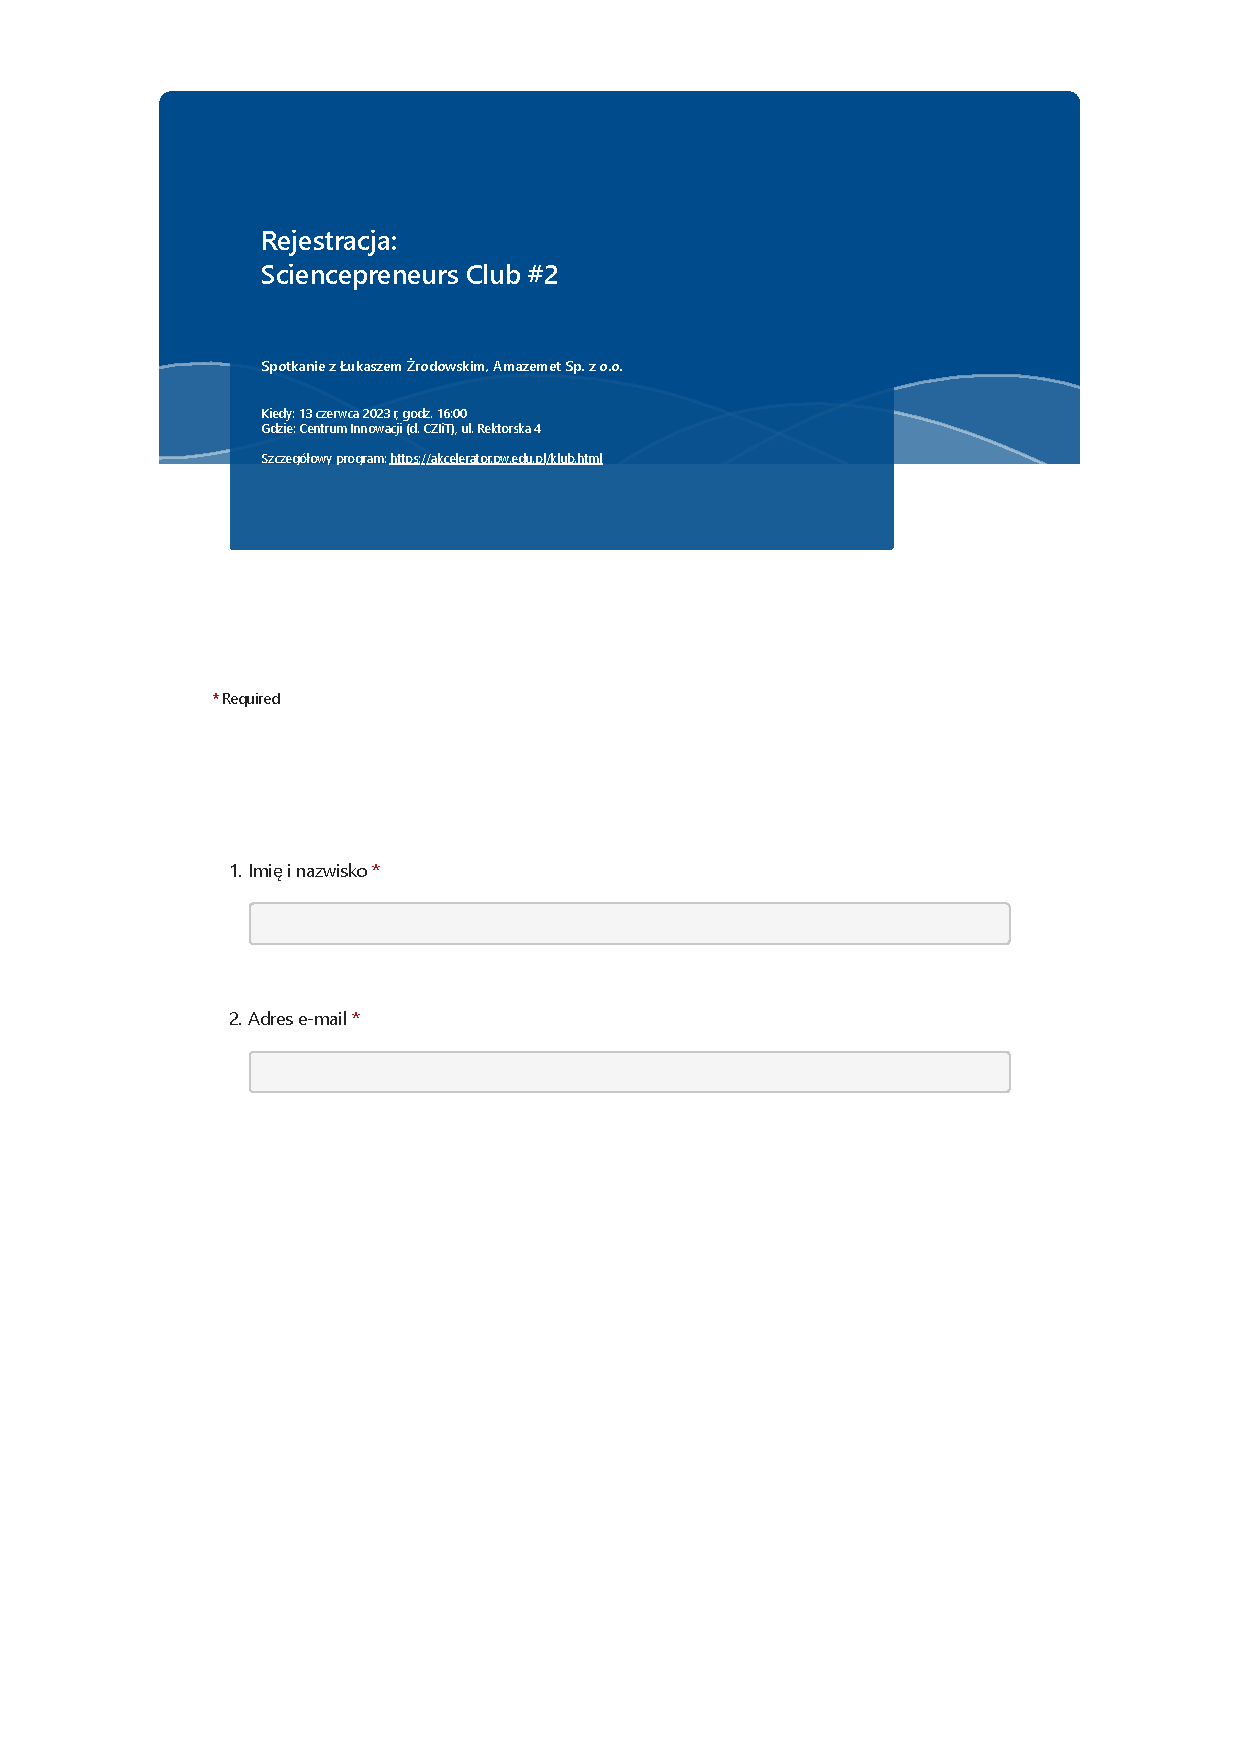
\includepdf[pages=-]{pdf/RejestracjaSciencepreneursClub2.pdf} % Wstawia PDF

% Trzeci załącznik
\chapter{Dodatkowe materiały cyfrowe}
\label{app:materialy}

Pełna konfiguracja systemu oraz instrukcja wideo dostępne są w wersji cyfrowej:  
\begin{itemize}
    \item \textbf{Instrukcja wideo aktualizacji bazy danych} -- plik \texttt{Instrukcja Wideo Aktualizacji \\Baz Danych.mov}
    
    \item \textbf{Baza danych Microsoft Excel} -- plik \texttt{SC BAZA.xlsx}
    
     \item \textbf{Pliki konfiguracji automatyzacji} -- plik \texttt{AktualizacjarejestracjiSC3(froms)dobazy\\(excel).zip}
\end{itemize}

Wszystkie wymienione materiały znajdują się na dołączonym nośniku USB.